%%%%%%
%% Generic model
%%
\subsection{Model-independent signal shapes}
\label{sec:generic_models}

The SME predicts $n$th-order sinusoidal temporal oscillations of the forms
$\cos(n\omega_\oplus T_\oplus)$ and $\sin(n\omega_\oplus T_\oplus)$. Recall
from Sec.~\ref{ssec:SME} that a dimension $d$ SME operator is multiplied
by a coefficient of dimension $4-d$. A given coefficient induces a tower of 
$n$-order sidereal harmonics $n\omega_\oplus T_\oplus$ 
the number of Lorentz indices of an SME coefficient. 
For example, revisiting again ${\cal L}_b$ from Eq.~\eqref{bterm},
the SME coefficient $b_\mu$ has one Lorentz index. We showed 
in Eq.~\eqref{ATLAScomps} that only $n=1$ and 
$\cos(\omega_\oplus T_\oplus), \sin(\omega_\oplus T_\oplus)$ appear. 
For the $c$- and $d$-type coefficients, with two Lorentz indices, 
we expect $n=1$ and $n=2$ harmonics. This is observed in the 
decomposition of $c_f^{33}$ in Eq.~\eqref{c33}. 
Note that unique linear combinations of SME coefficients (prefactors) are
associated to a single harmonic of order $n$~\cite{Kostelecky:2009zp}.
There are no ``cross terms"
involving, for example, a prefactor with time-dependent
behavior controlled by both $\cos(\omega_\oplus T_\oplus)$ 
and $\cos(2\omega_\oplus T_\oplus)$. This is a generic
result applying for all $n$.

For the $a^{(5)}$- and $b^{(5)}$-type coefficients 
one finds $n=1, 2$ and $3$ harmonics in general.
The $a^{(5)}$ predictions for the Drell-Yan cross section
evaluated in the ATLAS detector frame are found to be absent 
$3\omega_\oplus$ signatures. This contrasts with 
the cross section for deep inelastic scattering, 
where all harmonics appear.
An intuitive explanation for this 
absence is that Drell-Yan is
a more colliear or ``symmetric" process 
than deep inelastic scattering.
As a result, fewer coefficient components 
are present in the detector-frame
cross section. The ones that do appear have 
laboratory indices which, upon replacing with the SCF coefficients,
exhibit only first and second harmonics.
This is likely to be a special case
rather than a generic expectation for Drell-Yan.
A significant number of nonminimal 
SME coefficients of low mass 
dimension (e.g. $d=5,6$) have distinct
symmetry properties relative to those exhibited by
the $a^{(5)}$-type coefficients. 
Anticipating that phenomenological predictions
with higher than $2\omega_\oplus$ harmonics
will appear in future provides motivation 
for developing the generic framework outlined here.

In this section, we outline a new method for capturing
higher-order harmonics that encompass 
any new physics associated with sidereal oscillations. 
While the SME is a model-independent effective field theory, it makes
specific predictions about the prefactors multiplying the 
sidereal functions. We generalize these types of signal shapes
by leaving the prefactors as free fit parameters. 

In particular, we consider three distinct generic 
model signal shapes 
%
\begin{subequations}
\label{eq:generic_shapes}
\begin{align}
    f_{1}(\omega_\oplus T_\oplus| p_{1}, p_{2}) 
    &= 1+ p_{1}
    \cos(\omega_\oplus T_\oplus) 
    + p_{2}\sin(\omega_\oplus T_\oplus), \label{eq:generic_shape1} \\
    f_{2}(2\omega_\oplus T_\oplus| p_{1}, p_{2}) 
    &= 1+ p_{1}\cos(2\omega_\oplus T_\oplus) 
    + p_{2}\sin(2\omega_\oplus T_\oplus), \label{eq:generic_shape2} \\
    f_{3}(3\omega_\oplus T_\oplus| p_{1}, p_{2}) 
    &= 1+ p_{1}\cos(3\omega_\oplus T_\oplus) 
    + p_{2}\sin(3\omega_\oplus T_\oplus), \label{eq:generic_shape3}
\end{align}
\end{subequations}
%
and treat each function $f_1, f_2$ and $f_3$ with prefactor parameters
$p_1$ and $p_2$ as mutually exclusive. As we limit
attention to a finite number of free parameters, and make no assumption 
about the physics generating them, we refer to them as ``generic models". 
Parameters $p_1$ and $p_2$ are to be determined from $\chi^{2}$
fits to data. The results of these fits are the parameter values and a covariance matrix.
The corresponding $p_1$ and $p_2$ confidence intervals are obtained
from the covariance matrix.

%%% Should I write chi2 fits?
%Unlike SME models, the generic model has two free parameters to be determined 
%from fit to data by applying two parametric $\chi^{2}$ fits. The fit result 
%would be values $p_{1}$, $p_{2}$ and covariance matrix. Confidence interval 
%for $p_{1}$ and $p_{2}$ are obtained from the corresponding covariance matrix.


\subsection{Spurious signal uncertainties on $p_{1}$ and $p_{2}$}
%%% fit to 10K scrambled datasets.
%%% fit results

Figure~\ref{fig:real_data_scrambled_Generic_combined_fit} shows the estimated 
set of parameters, $p_{1}$ and $p_{2}$, corresponding to generic models with 
different frequencies, 
$\omega_\oplus T_\oplus$, $2\omega_\oplus T_\oplus$, 
$3\omega_\oplus T_\oplus$. These results 
are obtained from 10000 scrambled datasets by fitting each dataset with 
the generic signal shapes. 
The three signal shapes are mutually exclusive, 
so a fit includes one signal shape at a time. 
The corresponding numerical values 
of the Fig.~\ref{fig:real_data_scrambled_Generic_combined_fit} are also given 
in the Tab.~\ref{table:real_data_scrambled_Generic_combined_fit}.

In the ideal case, 
we could expect the central value of the parameters to be zero
because we took an average of the 10000 fit results from the scrambled datasets.
In reality, the average values are not zero, as we have seen in
Fig.~\ref{fig:real_data_scrambled_Generic_combined_fit}.  
Therefore, we can take 
these non-zero values as spurious signal 
uncertainties and include them in the unblinded results.

\begin{figure}
\centering
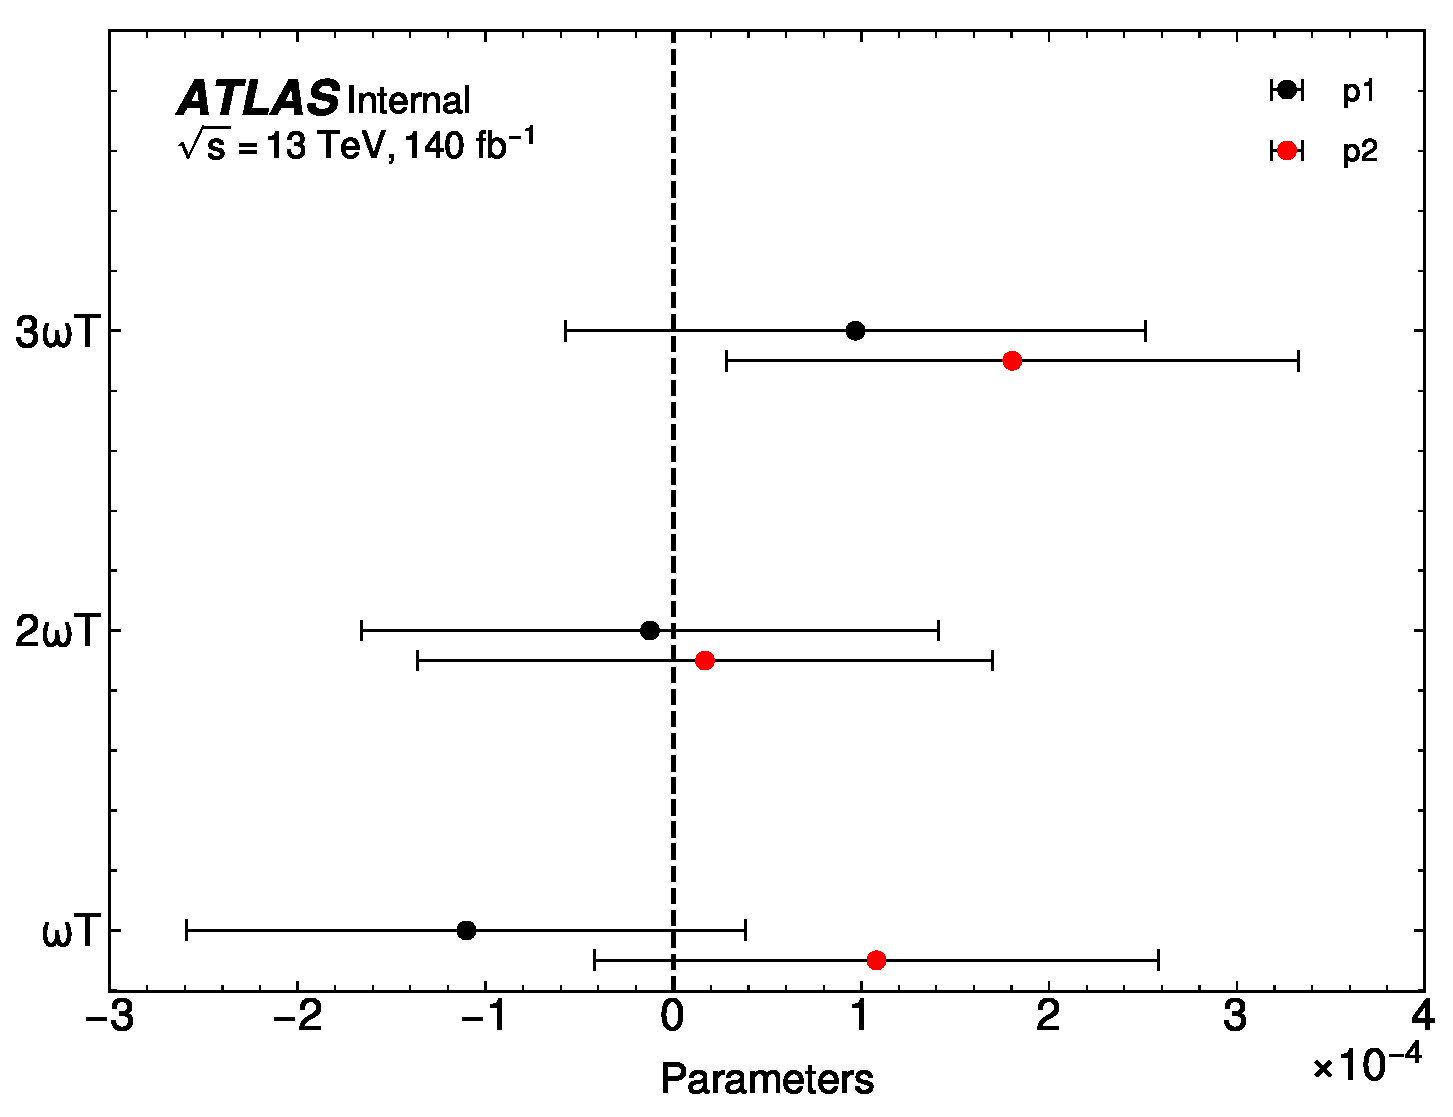
\includegraphics[width=0.75\textwidth]{figs/partially_unblinded_results/sig_config_6013_sidereal_combined_SciPy_generic}
\caption{Estimated parameters and their 
uncertainties of generic signal shapes; 
obtained by fitting 10000 scrambled datasets. 
The plot shows the mean and 
one standard deviation of 10000 fit results.
Note $\omega T = \omega_\oplus T_\oplus$ on the $y$-axis.}
\label{fig:real_data_scrambled_Generic_combined_fit}
\end{figure}

%%%%
%%% Sys table
%%%%
%%%%%%%%%%%%%%%
%%ee channel%%%
%%%%%%%%%%%%%%%
\begin{table}[hp]
\begin{center}
\color{gray}
%\resizebox{\textwidth}{!}{
\begin{tabular}{|l|c| c| c|}
\hline
  & \multicolumn{3}{|c|}{Generic models}\\
\hline
 Pars & $\omega_\oplus T_\oplus$ & $2\omega_\oplus T_\oplus$ & $2\omega_\oplus T_\oplus$\\
 \hline
$p_{1}$ & -1.10e-04 $\pm$ 1.49e-04 & -1.25e-05 $\pm$  1.54e-04 & 9.69e-05 $\pm$  1.54e-04\\
\hline
$p_{2}$ & 1.08e-04 $\pm$ 1.50e-04 & 1.68e-05 $\pm$ 1.53e-04 & 1.80e-04 $\pm$ 1.52e-04\\
\hline
\hline
\end{tabular}
%}
\color{black}

%\resizebox{\textwidth}{!}{
\begin{tabular}{|l|c| c| c|}
  \hline
    & \multicolumn{3}{|c|}{Generic models}\\
  \hline
   Pars & $\omega_\oplus T_\oplus$ & $2\omega_\oplus T_\oplus$ & $2\omega_\oplus T_\oplus$\\
   \hline
  $p_1$ & $(-1.23 \pm 1.49)\times 10^{-4}$ & $(-0.25 \pm 1.54)\times 10^{-4}$ & $(0.84 \pm 1.54)\times 10^{-4}$ \\
  \hline
  $p_2$ & $(1.08 \pm 1.50)\times 10^{-4}$ & $(0.16 \pm 1.53)\times 10^{-4}$ & $(1.79 \pm 1.52)\times 10^{-4}$ \\
  \hline
  $\text{corr}(p_1,p_2)$ & $0.0014$ & $-0.00086$ & $0.0071$ \\
  \hline
  \hline
  \end{tabular}
 % }
\end{center}
\caption{Estimated parameters and their 
uncertainties of generic signal shapes; 
obtained by fitting 10000 scrambled datasets. 
The means and one standard deviation of the 10000 fit results.}
\label{table:real_data_scrambled_Generic_combined_fit}
\end{table}
%

\subsection{Profiled $\chi^{2}$ fit with generic models}
% introduce spurious signal uncertainty size, s1 and s2
% introduce normal gaussian nuisance, b1, b2
% F(x, p1, p1,| b1, b2) = f(x, p1+b1*s1, p2+b2*s2)
Here we introduce, $s_{1}$ and $s_{2}$ 
as size of spurious signal uncertainties
corresponds to the parameters 
$p_{1}$ and $p_{2}$. The values of $s_{1}$ and 
$s_{2}$ are the absolute values of 
$p_{1}$ and $p_{2}$ in the 
Table~\ref{table:real_data_scrambled_Generic_combined_fit}, 
as these values are obtained from scrambled 
datasets (we take these samples as signal-free datasets). 

To add spurious signal uncertainties to the $\chi^{2}$ fit, 
we rewrite the Eqs.~\eqref{eq:generic_shapes} as
\begin{equation}
F(\omega_\oplus T_\oplus,\ p_1,\ p_2| \beta_{1},\ \beta_{2}) 
= f(\omega_\oplus T_\oplus,\ p_1+\beta_{1}*s_1, \ p_2+\beta_{1}*s_2), 
\end{equation}
where $\beta_{1}$ and $\beta_{2}$ nuisance parameters constrained as they
follow normal Gaussian centered at zero, 
and the standard deviation is one. 
$s_{1}$ and $s_{2}$ are constant in the equations.
The profiled $\chi^{2}$ fit is constructed using the function 
$F(\omega_\oplus T_\oplus,\ p_1,\ p_2| \beta_{1},\ \beta_{2})$. 




\subsection{Application of generic results}

In this subsection we show that the 
model-independent constraints in 
Eqs.~(\ref{eq:generic_shape1}--\ref{eq:generic_shape3}), 
together with the theory predictions given in 
Sec.~\ref{subsec:WC} 
(see Eqs.~(\ref{eq:SME coefficient functions}-\ref{eqn:14})) 
allow to reproduce the results of the 
one-parameter fits presented in Table~\ref{table:scrambel_results_10K}.

The starting point are the model-independent 
fits for the parameters $(p_1,p_2)$ summarized in 
Table~\ref{table:real_data_scrambled_Generic_combined_fit}. 
Adopting a simple frequentist $\chi^2$ fit 
based on the theoretical expressions in 
Sec.~\ref{subsec:WC} we obtain the 
results in Table~\ref{table:Direct_vs_Indirect_Comparison}, 
where, for ease of comparison, we show 
direct and indirect determinations side 
by side (the former are taken directly from 
Table~\ref{table:scrambel_results_10K}).

We see that the two procedures yield perfectly compatible results. 
Figure~\ref{fig:direct_indirect_results} shows the direct and indirect
 results in a plot for visualization.

\begin{table}[hp]
  \begin{center}
%  \resizebox{\textwidth}{!}{
  \begin{tabular}{|l|c|c|}
    \hline
    \hline
    Parameters & Direct & Indirect \\
    \hline
    $d_{\it u}^{\it X,Z}$ & $-(2.99 \pm 3.62)\times 10^{-6}$& $-(3.02 \pm 3.62)\times 10^{-6}$ \\
    \hline
    $d_{\it u}^{\it Y,Z}$ & $-(2.50 \pm 3.59)\times 10^{-6}$ & $-(2.55 \pm 3.59)\times 10^{-6}$\\
    \hline
    $d_{\it u}^{\it XY,XY}$ & $-(0.24 \pm 1.89)\times 10^{-6}$ &  $-(0.24 \pm 1.89)\times 10^{-6}$\\
    \hline
    $d_{\it u}^{\it X,Y}$ & $(1.41 \pm 9.40)\times 10^{-7}$ & $(1.40 \pm 9.41)\times 10^{-7}$\\
    \hline
    $c_{\it u}^{\it X,Z}$ & $-(2.32 \pm 2.81)\times 10^{-6}$ & $-(2.35 \pm 2.81)\times 10^{-6}$\\
    \hline
    $c_{\it u}^{\it Y,Z}$ & $-(1.94 \pm 2.79)\times 10^{-6}$ & $-(1.98 \pm 2.79)\times 10^{-6}$\\
    \hline
    $c_{\it u}^{\it XY,XY}$ &  $-(0.19 \pm 1.47)\times 10^{-6}$ &  $-(0.19 \pm 1.47)\times 10^{-6}$\\
    \hline
    $c_{\it u}^{\it X,Y}$ &  $(1.09 \pm 7.31)\times 10^{-7}$ & $(1.09 \pm 7.31)\times 10^{-7}$\\
    \hline
    $c_{\it d}^{\it X,Z}$ & $-(1.03 \pm 1.25)\times 10^{-4}$ &$-(1.05 \pm 1.25)\times 10^{-4}$ \\
    \hline
    $c_{\it d}^{\it Y,Z}$ & $-(0.87 \pm 1.24)\times 10^{-4}$ & $-(0.82 \pm 1.24)\times 10^{-4}$\\
    \hline
    $c_{\it d}^{\it XY,XY}$ & $-(0.83 \pm 6.54)\times 10^{-5}$ & $-(0.82 \pm 6.54)\times 10^{-5}$\\
    \hline
    $c_{\it d}^{\it X,Y}$ & $(0.49 \pm 3.25)\times 10^{-5}$ & $(0.49 \pm 3.26)\times 10^{-5}$ \\
    \hline
    \hline
    \end{tabular}
  %  }
  \end{center}
  \caption{Comparison between the direct 
  and indirect (using the results of the 
  two-parameter fits) extraction of 
  bounds on the $c$- and $d$-coefficients.}
  \label{table:Direct_vs_Indirect_Comparison}
  \end{table}
  %

  \begin{figure}[!h]
    \centering
    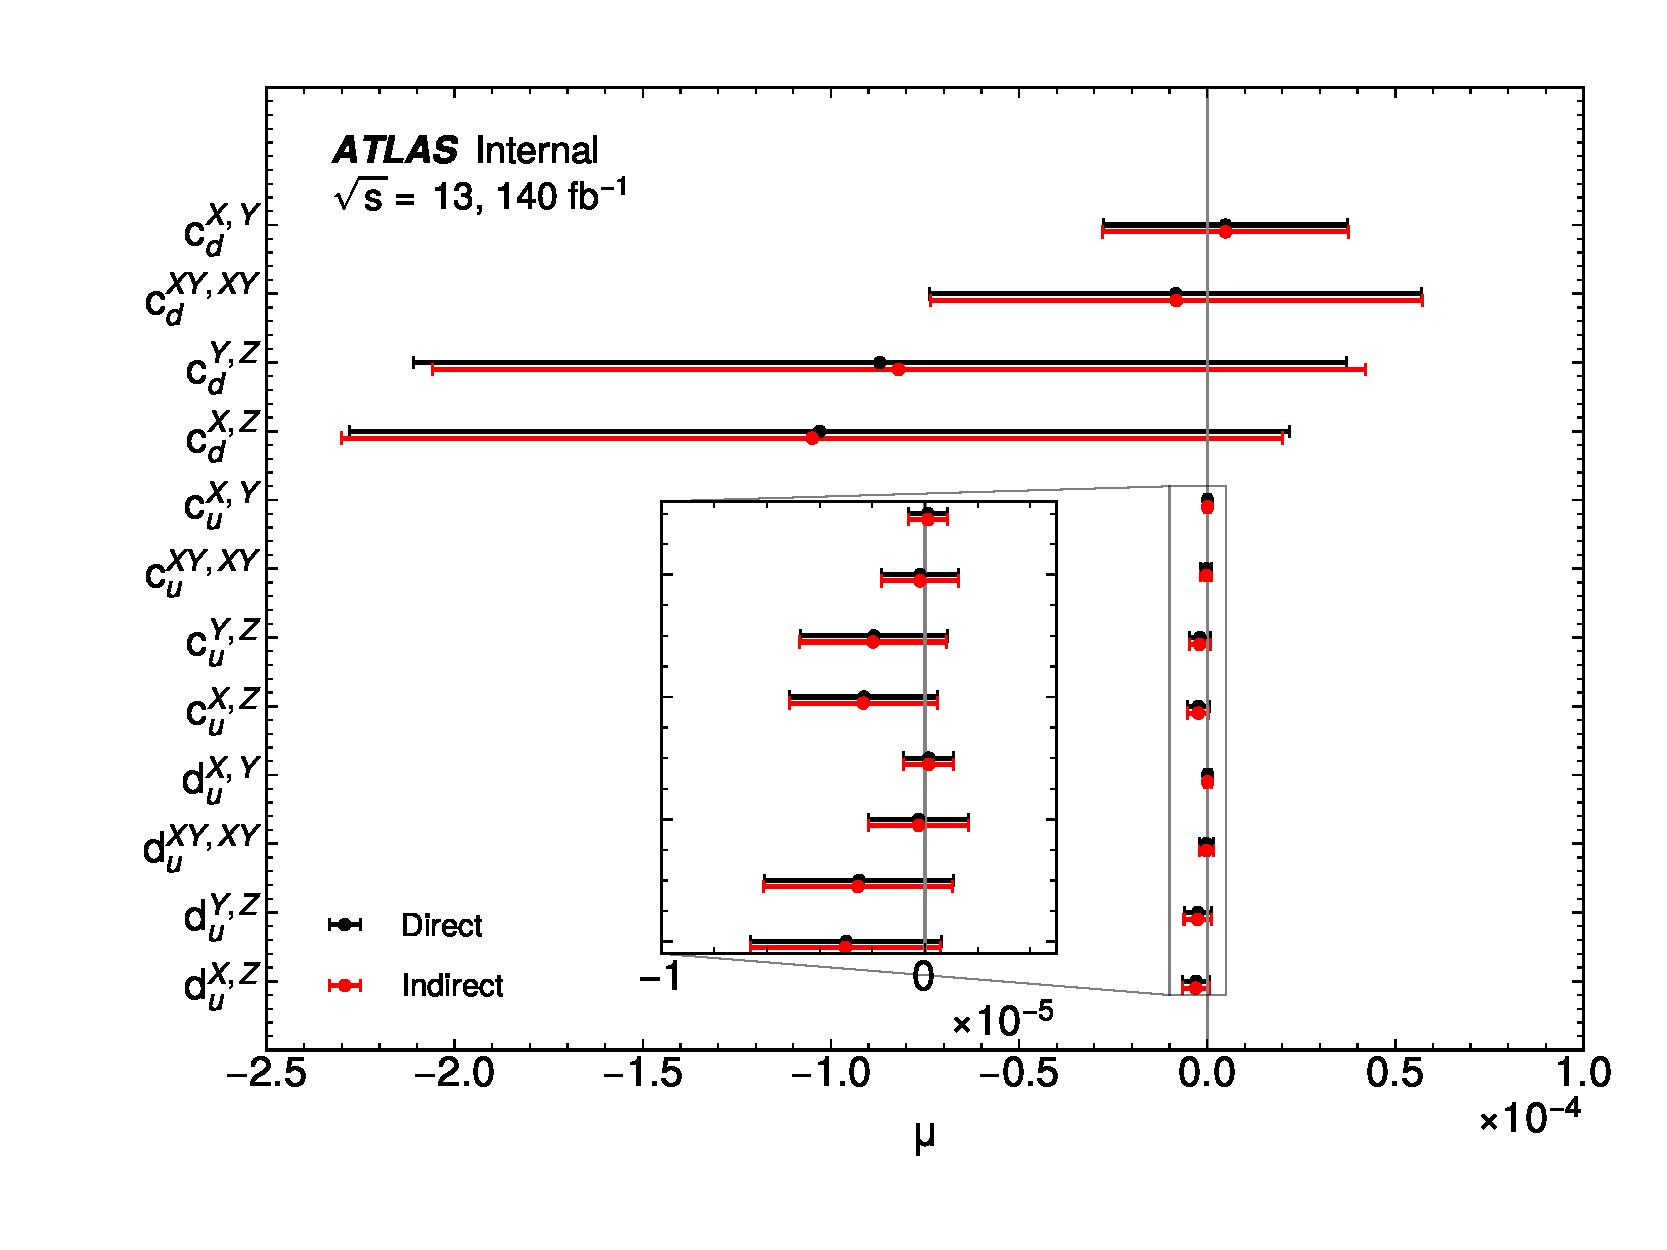
\includegraphics[width=0.75\textwidth]{figs/partially_unblinded_results/direct_indirect_test_results}
    \caption{
      Comparison of the direct (fit results of SME predictions) 
      and indirect (obtained using results of generic models).
      The indirect results are consistent with the direct results.
      Uncertainties correspond to 68\% (one-sigma) confidence intervals.
    }
    \label{fig:direct_indirect_results}
    \end{figure}
  

\subsection{Disentangling coefficient degeneracies}
\label{ssec:disentangle}

We briefly discuss the possibility of detecting a degenerate signal,
meaning one where at least two SME coefficients
could contribute to the signal.
Recall Eqs.~\eqref{eq:SME coefficient functions} and, for definiteness,
consider a scenario where the signal matches ``opposite phase" 
single-harmonic oscillations in the $u$-quark sector. 
For the minimal $c$- and $d$-type 
coefficients there are two possibilities:
\begin{align}
&d_u^{XZ}\left[6.28069\cos(\omega_\oplus T_\oplus)
-41.0569 \sin(\omega_\oplus T_\oplus)\right], \nonumber \\
&c_u^{XZ}\left[8.084\cos(\omega_\oplus T_\oplus)
-52.8451 \sin(\omega_\oplus T_\oplus)\right]
\end{align}
The small difference in magnitudes is a factor of 1.287.
Both coefficients can contribute to the signal, but 
a single measurement at $Q=m_Z$ can 
not distinguish between the possibilities: a $d_u$ dominated one, 
a $c_u$ dominated one, or some combination of the two.
A way to disentangle the signal 
is to perform another measurement at a different $Q$ value.
Referring to Fig.~\ref{fig:coeff_bounds}, one observes
that the $c_u$-type coefficient curve in red and
the $d_u$-type coefficient curve in green display distinct
patterns of sensitivity as $Q$ varies. 
The sensitivity to $c_u$ increases from around 
70 GeV and below, whereas $d_u$ 
decreases from $m_Z$ down to about 40 GeV. 
Focusing on the 40-45 GeV bin, the sensitivity
to $c_u$ decreases by about one order of magnitude, 
whereas $d_u$ about three orders of magnitude (both relative to $Q=m_Z$).
If the signal strengths measured at $Q=m_Z$ 
and $Q=40-45$\;GeV are found to differ by roughly an order of magnitude, 
this would disfavor the $d_u$-dominated scenario. This would suggest
that Lorentz violation couples more strongly 
to the $L+R$ chiral combination, which is the combination
that leaves the $u$-quark polarization properties unaffected.

